\subsection{\texorpdfstring{\(E_{7}\) 型系统}{E\_7 型系统}}

\begin{enumerate}
\def\labelenumi{(\Roman{enumi})}
\tightlist
\item
  以及 (II) 设 \(E = R^{8}\)，并令 \(R_{8}\) 为第 10 号在 E 中构造的根系。令 V 为 E 中由根 \(\alpha_{1}, \ldots, \alpha_{7}\)（它们属于 \(R_{8}\)）生成的超平面；它与第八个基本权 \(\omega = \varepsilon_{7} + \varepsilon_{8}\)（属于 \(R_{8}\)）正交。
\end{enumerate}

  令 \(R = R_{8} \cap V\)。则 \(R\) 是一个以 \((\alpha_{1}, \ldots, \alpha_{7})\) 为基的约化根系，参见 § 1，第 7 号，命题 20 的推论 4；因此，该系统为 \(E_{7}\) 型。其元素为：

\[
\begin{array}{c} \pm \varepsilon_ {i} \pm \varepsilon_ {j} (1 \leqslant i < j \leqslant 6), \quad \pm (\varepsilon_ {7} - \varepsilon_ {8}), \\ \pm \frac {1}{2} (\varepsilon_ {7} - \varepsilon_ {8} + \sum_ {i = 1} ^ {8} (- 1) ^ {\nu (i)} \varepsilon_ {i}) \quad \text { with } \sum_ {i = 1} ^ {8} \nu (i) \text { odd }. \end{array}
\]

根的数目为 \(n = 2 + \binom{6}{2}.4 + 2^6 = 126\)。正根为

\[
\pm \varepsilon_ {i} + \varepsilon_ {j} (1 \leqslant i <   j \leqslant 6). - \varepsilon_ {7} + \varepsilon_ {8},
\]

\[
\frac {1}{2} \left(- \varepsilon_ {7} + \varepsilon_ {8} + \sum_ {i = 1} ^ {6} (- 1) ^ {\nu (i)} \varepsilon_ {i}\right) \quad \text { with } \sum_ {i = 1} ^ {6} \nu (i) \text { odd }.
\]

\begin{enumerate}
\def\labelenumi{(\Roman{enumi})}
\setcounter{enumi}{2}
\item
  我们有 \(h = \frac{n}{l} = 18\)。
\item
  令 \(\tilde{\alpha} = \varepsilon_8 - \varepsilon_7 = 2\alpha_1 + 2\alpha_2 + 3\alpha_3 + 4\alpha_4 + 3\alpha_5 + 2\alpha_6 + \alpha_7\)，这是一个根。相对于 \((\alpha_i)\)，它的坐标之和为 \(17 = h - 1\)。因此它是最高根。它与 \(\alpha_i\)（\(2 \leqslant i \leqslant 7\)）正交，且 \((\tilde{\alpha}|\alpha_1) = 1\)。扩展 Dynkin 图为
\end{enumerate}

\pandocbounded{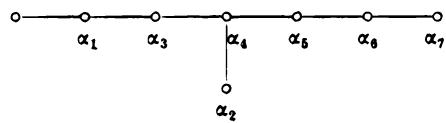
\includegraphics[keepaspectratio]{images/part002_8927380c.jpg}}

\begin{enumerate}
\def\labelenumi{(\Alph{enumi})}
\setcounter{enumi}{21}
\tightlist
\item
  由于 \((\alpha |\alpha) = 2\) 对所有 \(\alpha \in \mathbb{R}\) 成立，所以 \(R^{\prime} = R\)。
\end{enumerate}

对于 \(\Phi_{\mathrm{R}}\)，根的长度平方为 \(\frac{1}{18}\)，所以

\[
\Phi_ {\mathrm{R}} (x, y) = (x | y) / 36, \quad \text { and } \quad \gamma (\mathrm{R}) = 2 ^ {2}. 3 ^ {4}
\]

（§ 1，第 12 号，公式 (20)）。

\begin{enumerate}
\def\labelenumi{(\Roman{enumi})}
\setcounter{enumi}{5}
\tightlist
\item
  计算基本权得到
\end{enumerate}

\[
\begin{array}{r l} & {\omega_ {1} = \varepsilon_ {8} - \varepsilon_ {7} = 2 \alpha_ {1} + 2 \alpha_ {2} + 3 \alpha_ {3} + 4 \alpha_ {4} + 3 \alpha_ {5} + 2 \alpha_ {6} + \alpha_ {7}} \\ & {\omega_ {2} = \frac {1}{2} (\varepsilon_ {1} + \varepsilon_ {2} + \varepsilon_ {3} + \varepsilon_ {4} + \varepsilon_ {5} + \varepsilon_ {6} - 2 \varepsilon_ {7} + 2 \varepsilon_ {8})} \\ & {\qquad = \frac {1}{2} (4 \alpha_ {1} + 7 \alpha_ {2} + 8 \alpha_ {3} + 12 \alpha_ {4} + 9 \alpha_ {5} + 8 \alpha_ {6} + 3 \alpha_ {7})} \\ & {\omega_ {3} = \frac {1}{2} (- \varepsilon_ {1} + \varepsilon_ {2} + \varepsilon_ {3} + \varepsilon_ {4} + \varepsilon_ {5} + \varepsilon_ {6} - 3 \varepsilon_ {7} + 3 \varepsilon_ {8})} \\ & {\qquad = 3 \alpha_ {1} + 4 \alpha_ {2} + 6 \alpha_ {3} + 8 \alpha_ {4} + 6 \alpha_ {5} + 4 \alpha_ {6} + 2 \alpha_ {7}} \\ & {\omega_ {4} = \varepsilon_ {3} + \varepsilon_ {4} + \varepsilon_ {5} + \varepsilon_ {6} + 2 (\varepsilon_ {8} - \varepsilon_ {7})} \\ & {\qquad = 4 \alpha_ {1} + 6 \alpha_ {2} + 8 \alpha_ {3} + 12 \alpha_ {4} + 9 \alpha_ {5} + 6 \alpha_ {6} + 3 \alpha_ {7}} \\ & {\omega_ {5} = \varepsilon_ {4} + \varepsilon_ {5} + \varepsilon_ {6} + \frac {3}{2} (\varepsilon_ {8} - \varepsilon_ {7})} \\ & {\qquad = \frac {1}{2} (6 \alpha_ {1} + 9 \alpha_ {2} + 12 \alpha_ {3} + 18 \alpha_ {4} + 15 \alpha_ {5} + 10 \alpha_ {6} + 5 \alpha_ {7})} \\ & {\omega_ {6} = \varepsilon_ {5} + \varepsilon_ {6} - \varepsilon_ {7} + \varepsilon_ {8}} \\ & {\qquad = 2 \alpha_ {1} + 3 \alpha_ {2} + 4 \alpha_ {3} + 6 \alpha_ {4} + 5 \alpha_ {5} + 4 \alpha_ {6} + 2 \alpha_ {7}} \\ & {\omega_ {7} = \varepsilon_ {6} + \frac {1}{2} (\varepsilon_ {8} - \varepsilon_ {7})} \\ & {\qquad = \frac {1}{2} (2 \alpha_ {1} + 3 \alpha_ {2} + 4 \alpha_ {3} + 6 \alpha_ {4} + 5 \alpha_ {5} + 4 \alpha_ {6} + 3 \alpha_ {7}).} \end{array}
\]

\begin{enumerate}
\def\labelenumi{(\Roman{enumi})}
\setcounter{enumi}{6}
\tightlist
\item
  正根之和 \(2\rho\) 等于 \(2\sum_{i=1}^{7}\omega_i\)（§ 1，第 10 号，命题 29），所以
\end{enumerate}

\[
\begin{array}{r l} 2 \rho & = 2 \varepsilon_ {2} + 4 \varepsilon_ {3} + 6 \varepsilon_ {4} + 8 \varepsilon_ {5} + 10 \varepsilon_ {6} - 17 \varepsilon_ {7} + 17 \varepsilon_ {8} \\ & = 34 \alpha_ {1} + 49 \alpha_ {2} + 66 \alpha_ {3} + 96 \alpha_ {4} + 75 \alpha_ {5} + 52 \alpha_ {6} + 27 \alpha_ {7}. \end{array}
\]

\begin{enumerate}
\def\labelenumi{(\Roman{enumi})}
\setcounter{enumi}{7}
\tightlist
\item
  由第 10 号 (VIII) 及 § 1，第 10 号，命题 28，有
\end{enumerate}

\[
\mathrm{Q} (\mathrm{R}) = \mathrm{Q} (\mathrm{R} _ {8}) \cap \mathrm{V} = \mathrm{L} _ {3} \cap \mathrm{V} \quad \text { and } \quad \mathrm{P} (\mathrm{R}) = p (\mathrm{P} (\mathrm{R} _ {8})) = p (\mathrm{L} _ {3}),
\]

其中 p 表示 E 到 V 的正交投影。群 \(Q(R)\) 的基为 \((\alpha_{1},\ldots,\alpha_{7})\)；群 \(P(R)\) 由 \(Q(R)\) 和

\[
p (\alpha_ {8}) = \alpha_ {8} - \frac {1}{2} \omega .
\]

我们有 \(\omega\in\mathrm{P}(\mathrm{R}_{8})\)，\(\frac{1}{2}\omega\notin\mathrm{P}(\mathrm{R}_{8})\)，所以 \(2p(\alpha_{8})\in\mathrm{Q}(\mathrm{R})\) 而 \(p(\alpha_{8})\notin\mathrm{Q}(\mathrm{R})\)。因此，\(\mathrm{P}(\mathrm{R})/\mathrm{Q}(\mathrm{R})\) 同构于 Z/2Z，并由例如 \(\omega_{7}\) 的像生成。

连接指标为 2。

\begin{enumerate}
\def\labelenumi{(\Roman{enumi})}
\setcounter{enumi}{8}
\tightlist
\item
  \(W(R)\) 的指数序列有 7 项。与 \(h = 18\) 互素的数 1、5、7、11、13、17 出现在此序列中。最后一个指数 \(m\) 必须满足 \(m + m = 18\)（第 V 章，§ 6，第 2 号，公式 (2)）。因此，指数序列为
\end{enumerate}

\[
1, 5, 7, 9, 11, 13, 17.
\]

\begin{enumerate}
\def\labelenumi{(\Alph{enumi})}
\setcounter{enumi}{23}
\tightlist
\item
  由 (IX) 及第 V 章 § 6 第 2 号命题 3 的推论 1，得到 W(R) 的阶为
\end{enumerate}

\[
2. 6. 8. 10. 12. 14. 18 = 2 ^ {10}. 3 ^ {4}. 5. 7.
\]

\begin{enumerate}
\def\labelenumi{(\Roman{enumi})}
\setcounter{enumi}{10}
\item
  Dynkin 图的唯一自同构是恒等自同构，所以 \(\mathbf{A}(\mathbf{R}) = \mathbf{W}(\mathbf{R})\) 且 \(w_0 = -1\)。
\item
  \(\mathrm{P}(\mathrm{R}^{-})/\mathrm{Q}(\mathrm{R}^{-})\) 只有一个非单位元。它互换对应于 \(\alpha_{0}\) 和 \(\alpha_{7}\)、\(\alpha_{1}\) 和 \(\alpha_{6}\)、\(\alpha_{3}\) 和 \(\alpha_{5}\) 的顶点，并固定 \(\alpha_{2}\) 和 \(\alpha_{4}\)。
\end{enumerate}

